\subsection{数学归纳法的应用举例}\label{subsec:2-5}

\liti 用数学归纳法证明
$$ 1^2 + 2^2 + 3^2 + \cdots + n^2 = \dfrac{n(n + 1)(2n + 1)}{6} \text{。} $$

\zhengming (1) 当 $n = 1$ 时,左边是 $1^2 = 1$,右边是 $\dfrac{1}{6} \cdot 1 \cdot 2 \cdot 3 = 1$,等式成立。

(2) 假设当 $n = k$ 时等式成立,就是
$$ 1^2 + 2^2 + 3^2 + \cdots + k^2 = \dfrac{k(k + 1)(2k + 1)}{6} \text{,} $$
那么,
\begin{align*}
      & 1^2 + 2^2 + 3^2 + \cdots + k^2 + (k + 1)^2 \\
    = & \dfrac{k(k + 1)(2k + 1)}{6} + (k + 1)^2 \\
    = & \dfrac{k(k + 1)(2k + 1) + 6(k + 1)^2}{6} \\
    = & \dfrac{(k + 1)(2k^2 + 7k + 6)}{6} \\
    = & \dfrac{(k + 1)(k + 2)(2k + 3)}{6} \\
    = & \dfrac{(k + 1)[(k + 1) + 1][2(k + 1) + 1]}{6} \text{。}
\end{align*}

这就是说,当 $n = k + 1$ 时等式也成立。

根据 (1) 和 (2),可知等式对任何 $n \in N$ 都成立。

\begin{wrapfigure}[10]{r}{5cm}
    \centering
    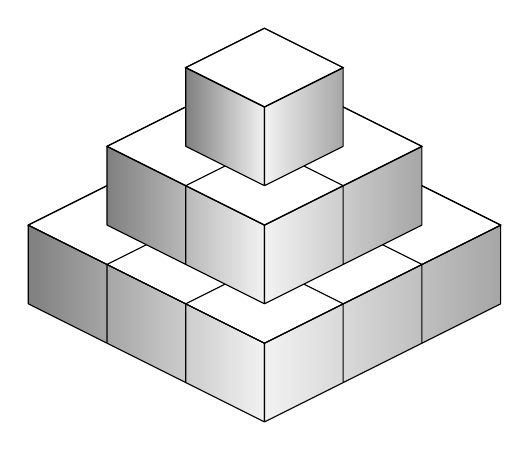
\begin{tikzpicture}
    \tikzset {
        cube layer/.pic = {
            \pgfmathsetmacro{\num}{#1}
            \shade[yslant=-0.5,right color=gray!10, left color=black!50] (0,0) rectangle +(\num,1);
            \draw [yslant=-0.5] (0,0) grid (\num,1);
            \shade[yslant=0.5,right color=gray!70,left color=gray!10] (\num,-\num) rectangle +(\num,1);
            \draw [yslant=0.5] (\num,-\num) grid (2*\num,1-\num);
            \draw [yslant=0.5,xslant=-1,fill=white] (1,1-\num) rectangle +(\num,\num);
            \draw [yslant=0.5,xslant=-1][fill=blue] (1,1-\num) grid (\num+1, 1);
        }
    }
    \path(0, 0) pic {cube layer=3};
    \path(1, 1) pic {cube layer=2};
    \path(2, 2) pic {cube layer=1};
\end{tikzpicture}
    \caption{}\label{fig:2-8}
\end{wrapfigure}

用这个公式可以计算如图 \ref{fig:2-8} 所示的一堆物品的总数。

\liti 用数学归纳法证明 $x^{2n} - y^{2n} \; (n \in N)$ 能被 $x + y$ 整除。

\zhengming (1) 当 $n = 1$ 时,$x^2 - y^2 = (x + y)(x - y)$ 能被 $x + y$ 整除。

(2) 假设当 $n = k\; (k \in N)$ 时,$x^{2k} - y^{2k}$ 能被 $x + y$ 整除,那么

\begin{align*}
      & x^{2(k+1)} - y^{2(k+1)} \\
    = & x^2 \cdot x^{2k} - y^2 \cdot y^{2k} \\
    = & x^2 \cdot x^{2k} - x^2 \cdot y^{2k} + x^2 \cdot y^{2k} - y^2 \cdot y^{2k} \\
    = & x^2(x^{2k} - y^{2k}) + y^{2k}(x^2 - y^2) \text{。}
\end{align*}

因为 $x^{2k} - y^{2k}$ 与 $x^2 - y^2$ 都能被 $x + y$ 整除,所以它们的和 $x^2(x^{2k} - y^{2k}) + y^{2k}(x^2 - y^2)$
也能被 $x + y$ 整除。这就是说,当 $n = k + 1$ 时,$x^{2(k+1)} - y^{2(k+1)}$ 能被 $x + y$ 整除。

根据 (1) 和 (2),可知命题对任何 $n \in N$ 都成立。


\liti 平面内有 $n$ 条直线,其中任何两条不平行,任何三条不过同一点,证明交点的个数 $f(n)$ 等于 $\dfrac{1}{2} n(n-1)$。

\zhengming (1) 当 $n = 2$ 时,两条直线的交点只有 $1$ 个,即 $f(2) = 1$。又当 $n = 2$ 时,
$$ \dfrac{1}{2} \times 2 \times (2 - 1) = 1 ,$$
因此命题成立。


\begin{wrapfigure}[10]{r}{7cm}
  \centering
  \begin{tikzpicture}
    \def \line(#1){a#1}
    \draw [name path=a1] (0, 0) -- (6.5,0);
    \draw [name path=a2] (0, -2.2) -- (6, 2.5);
    \draw [name path=a3] (1.3, -3.1) -- (3, 4);
    \draw [name path=a4] (5.6, -2.8) -- (2, 4);
    \draw [name path=a5] (6.7, -2.5) -- (0.2, 2.6);
    \foreach \x in {1,...,4} {
        \pgfmathtruncatemacro{\start}{\x+1}
        \foreach \y in {\start,...,5} {
            \filldraw [name intersections={of=\line(\x) and \line(\y), by=i}] (i) circle (0.1);
        }
    }

    \node at (1.7, 0.3) {$A_1$};
    \node at (2.5, 0.3) {$A_2$};
    \node at (4.3, 0.3) {$A_k$};
    \node at (6, 0.3) {$l$};
\end{tikzpicture}
  \caption{}\label{fig:2-9}
\end{wrapfigure}

(2) 假设 $n = k$ 时命题成立,就是说,平面内满足题设的任何 $k$ 条直线的交点的个数 $f(k)$ 等于 $\dfrac{1}{2} k(k - 1)$。
现在来考虑平面内有 $k + 1$ 条直线的情况。任取其中的 $1$ 条直线,记为 $l$ (图\ref{fig:2-9})。由上述归纳法的假设,
除 $l$ 以外的其他 $k$ 条直线的交点的个数 $f(k)$ 等于 $\dfrac{1}{2} k(k - 1)$ 。
另外,因为已知任何两条直线不平行,所以直线 $l$ 必与平面内其他 $k$ 条直线都相交;
又因为已知任何三条直线不过同一点,所以上面的 $k$ 个交点两两不相同,且与平面内其他的 $\dfrac{1}{2} k(k - 1)$ 个交点也两两不相同,
从而平面内交点的个数是

\begin{align*}
      & \dfrac{1}{2} k(k - 1) + k \\
    = & \dfrac{1}{2} k[(k - 1) + 2] \\
    = & \dfrac{1}{2} (k+1) [(k+1) - 1] \text{。}
\end{align*}

这就是说,当 $n=k+1$ 时, $k+1$ 条直线的交点个数 $f(k+1)$ 等于 $\dfrac{1}{2} (k+1) [(k+1) - 1]$ 。

根据 (1) 和 (2),可知命题对任何 $n \geqslant 2$ 且 $n \in N$ 都成立。


\liti 设 $\sin\dfrac{\alpha}{2} \neq 0$,用数学归纳法证明
$$ \sin \alpha + \sin 2\alpha + \sin 3\alpha + \cdots + \sin n\alpha = \dfrac{\sin \dfrac{n\alpha}{2} \sin \dfrac{(n+1)\alpha}{2}}{\sin \dfrac{\alpha}{2}} \text{。} $$

\zhengming (1) 当 $n = 1$ 时,左边是 $\sin\alpha$,右边是
$$ \dfrac{\sin \dfrac{\alpha}{2} \sin \alpha}{\sin \dfrac{\alpha}{2}} = \sin\alpha \text{,} $$
等式成立。

(2) 假设当 $n = k$ 时等式成立,就是
$$ \sin \alpha + \sin 2\alpha + \sin 3\alpha + \cdots + \sin k\alpha = \dfrac{\sin \dfrac{k\alpha}{2} \sin \dfrac{(k+1)\alpha}{2}}{\sin \dfrac{\alpha}{2}} \text{,} $$
那么,

\begin{align*}
      & \sin \alpha + \sin 2\alpha + \sin 3\alpha + \cdots + \sin k\alpha + \sin (k+1)\alpha \\
    = & \dfrac{\sin \dfrac{k\alpha}{2} \sin \dfrac{(k+1)\alpha}{2}}{\sin \dfrac{\alpha}{2}} + \sin (k+1)\alpha \\
    = & \dfrac{\sin \dfrac{k\alpha}{2} \sin \dfrac{(k+1)\alpha}{2} +  \sin \dfrac{\alpha}{2} \sin (k+1)\alpha}{\sin \dfrac{\alpha}{2}} \\
    = & \dfrac{\dfrac{1}{2} \left( \cos\dfrac{\alpha}{2} - \cos\dfrac{2k+1}{2}\alpha + \cos\dfrac{2k+1}{2}\alpha - \cos\dfrac{2k+3}{2}\alpha \right)}{\sin\dfrac{\alpha}{2}} \\
    = & \dfrac{\cos\dfrac{\alpha}{2} - \cos\dfrac{2k+3}{2}\alpha}{2\sin\dfrac{\alpha}{2}} \\
    = & \dfrac{\sin\dfrac{(k+1)\alpha}{2} \sin\dfrac{[(k+1)+1]\alpha}{2}}{\sin\dfrac{\alpha}{2}} \text{。}
\end{align*}

这就是说,当 $n = k + 1$ 时等式也成立。

根据 (1) 和 (2),可知等式对任何 $n \in N$ 都成立。


\lianxi

用数学归纳法证明:

\begin{xiaotis}

\xiaoti{$1 \cdot 2 + 2 \cdot 3 + 3 \cdot 4 + \cdots + n(n+1) = \dfrac{1}{3}n(n+1)(n+2)$。}

\xiaoti{$-1 + 3 - 5 + \cdots + (-1)^n (2n-1) = (-1)^n n$。}

\xiaoti{$x^n - y^n \; (n \in N)$ 能被 $x - y$ 整除。}

\xiaoti{凸 $n$ 边形的内角和 $f(n) = (n - 2) \pi \quad (n \geqslant 3)$。}

\end{xiaotis}

